\documentclass[a4paper]{article}

\usepackage[T1]{fontenc}
\usepackage[utf8]{inputenc}
\usepackage[english]{babel}
\usepackage{csquotes}
\usepackage{listings}
\usepackage{multicol}
\lstset{language=c,frame=single,captionpos=b}
\usepackage{hyperref}
\usepackage{amsmath}
\usepackage[backend=biber, sorting=none,maxbibnames=40]{biblatex}
\renewbibmacro{in:}{}
\addbibresource{ref.bib}
\usepackage{graphicx}
\usepackage{placeins}
\usepackage[margin=2.5cm]{geometry}
\usepackage{subcaption}
\usepackage[affil-it]{authblk}
\usepackage{color}
\usepackage{amssymb,amsmath}
\usepackage{subfloat}
\usepackage{float}

\begin{document}
\title{MPI Assignment: N-body Simulations}
\author{Stefano Sandonà}
\affil{Vrije Universiteit Amsterdam, Holland}
\date{}
		
\maketitle

\section{The N-body problem}
\label{sec:nbody_problem}
The N-body problem consists of the prediction of the individual motions of N celestial objects (bodies) with some properties (mass, initial velocity, radius, ...). This is done by measuring the force that they exert on each other (Coulomb gravity,...) and as a result, a simulation of the behavior of the system over time is obtained.  

\section{The sequential algorithm}
\label{sec:seq_algo}
The Listing \ref{simple} shows the simplified structure of the sequential algorithm.
\begin{lstlisting}[label=simple, caption=general sequential algorithm]
for each timestep do
	Compute forces between all bodies
	Compute new positions and velocities
\end{lstlisting}

As first thing, the time is discretized, so that the application knows what to do at certain time steps. After that, for each step, the algorithm computes the force between the bodies. With the result, the new velocity and position of all the bodies are updated.

\subsection{Force computation}
\label{sec:force_comp_seq}
This step of the algorithm is the most expensive and defines its complexity.
The force that bodies exert on each other has to be calculated once per pair of bodies (Listing \ref{forceloop}).
\begin{lstlisting}[label=forceloop, caption=loop for the force calculation]
for (b=0; b<bodyCt; ++b) {
		for (c=b+1; c<bodyCt; ++c) {
			...
\end{lstlisting}
With N bodies, there are \textit{(N-1)+(N-2)+(N-3)+...+1} pairs, so that \textit{O(N\textsuperscript{2})} force computations for every time step.

\section{Parallel N-body algorithm}
\label{sec:par}
An efficient parallelization of this algorithm is not trivial because for every step the updated information from all the bodies that are part of our system is needed in order to calculate the correct velocities and positions. The next paragraph was introduced to explain the technology used to develop the parallel implementation.

\subsection{MPI}
\label{sec:mpi}
For this project was used the Message Passing Interface (MPI), a message passing library that is developed and maintained by a consortium of academic, research, and industry partners, that can be added to sequential languages (C, Fortran) to program multiple nodes. Using this library, to set up a point-to-point or collective communication is simplified. In addition to High performance, network and process fault tolerance is provided, making this library optimal for the parallel programming. For the collective commmunication, lots of useful functions are provided, like the \textit{MPI\_Bcast} to send data to all processes, the \textit{MPI\_Gather} to gather data from all processes, the \textit{MPI\_Scatter} to scatter data to all processes and others.

\subsection{Work distribution}
\label{sec:bodies_distr}
One of the major problems of the parallel algorithms is the load imbalance. If the work is not fairly distributed among the machines involved in the computation, there will be some machines idle while the others will still work. This problem affects a lot the performance of an application because the overall execution time depends on the last machine that terminate the computation. 
Looking at this specific case, there were two possible ways to follow: a fair distribution of the bodies or a fair distribution of the forces to compute. The major differences between this 2 approaches were encountered when the amount of work to distribute was not perfectly divisible by the number of machines.
Using a simple \textit{for} construct (Listing \ref{fair}), it is possible to calculate the chunks of forces/bodies to assign to each computational node. The Figure \ref{fig:repa} shows two examples of repartition.

\begin{lstlisting}[label=fair, caption=fair distribution of work]
int sum = 0;
int rem = workAmount % numProcs; 
for (i = 0; i < numprocs; i++) {
    work_per_proc[i] = workAmount / numProcs;
    if (rem > 0) {
        work_per_proc[i]++;
        rem--;
    }
    displs[i] = sum;
    sum += work_per_proc[i];
}
\end{lstlisting}
\FloatBarrier

\begin{figure*}[!ht]
    \centering
    \begin{subfigure}[b]{0.5\textwidth}
        \centering
        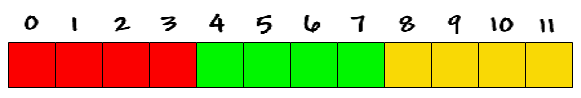
\includegraphics[width=1\linewidth]{array_procs_3}
        \caption{3 computational nodes}
        \label{fig:repa1}
    \end{subfigure}%
    ~ 
    \begin{subfigure}[b]{0.5\textwidth}
        \centering
        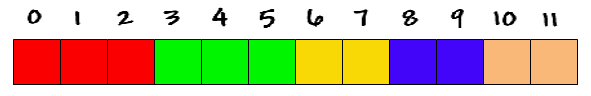
\includegraphics[width=1\linewidth]{array_procs_5}
        \caption{5 computational nodes}
        \label{fig:repa2}
    \end{subfigure}
    \caption{Repartition of 12 forces/bodies}
    \label{fig:repa}
    	
\end{figure*}
\FloatBarrier

A comparison of the two approaches was reported on the next paragraphs in order to clarify the made decisions.

\subsubsection{Approach 1 - Bodies repartition}
\label{sec:a1}

The total amount of bodies (known at the beginning) is distributed as fairly as possible among the  MPI processes as shown in the Listing \ref{fair}. Then, to avoid a duplication of work, given a pair of bodies chunks, half of the forces are calculated by one MPI node, and half by the other. The repartition is clarified in the Figures \ref{fig:pr1}, \ref{fig:pr2} and \ref{fig:pr3}.


\begin{figure}[!ht]
\centering
\begin{subfigure}{.3\textwidth}
  \centering
  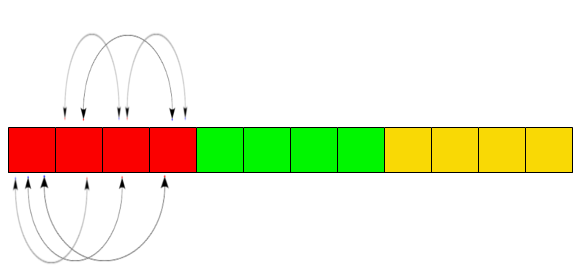
\includegraphics[width=1\linewidth]{array_proc_0_b_0}
\end{subfigure}%
\begin{subfigure}{.3\textwidth}
  \centering
  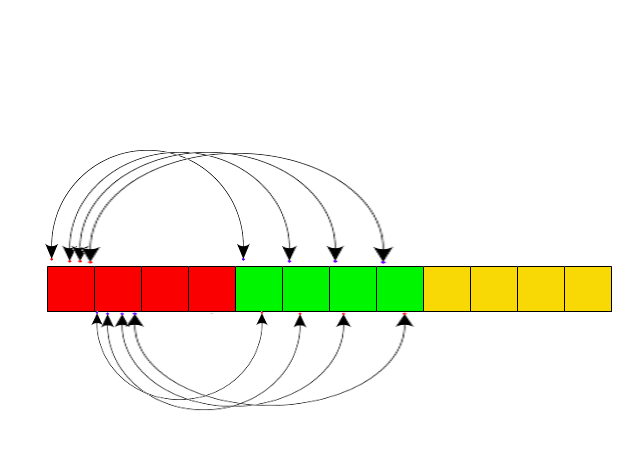
\includegraphics[width=1\linewidth]{array_proc_0_b_1}
\end{subfigure}\\ %
\begin{subfigure}{.3\textwidth}
  \centering
  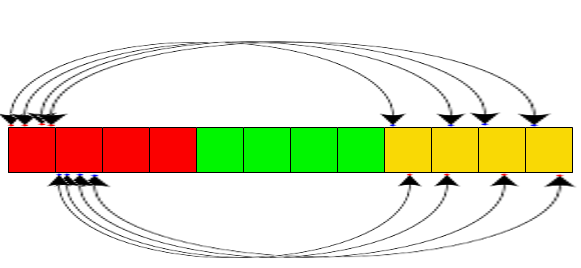
\includegraphics[width=1\linewidth]{array_proc_0_b_2}
\end{subfigure}
  \caption{Forces computed by Node 0 (6+8+8=22)}
  \label{fig:pr1}
\end{figure}
\FloatBarrier

\begin{figure}[!ht]
\centering
\begin{subfigure}{.3\textwidth}
  \centering
  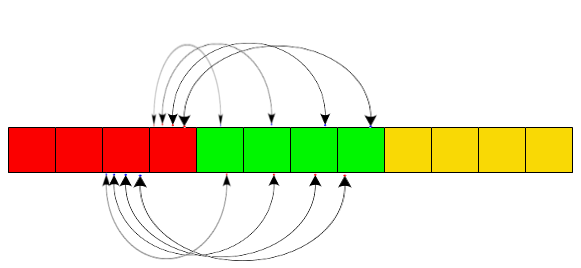
\includegraphics[width=1\linewidth]{array_proc_1_b_0}
\end{subfigure}%
\begin{subfigure}{.3\textwidth}
  \centering
  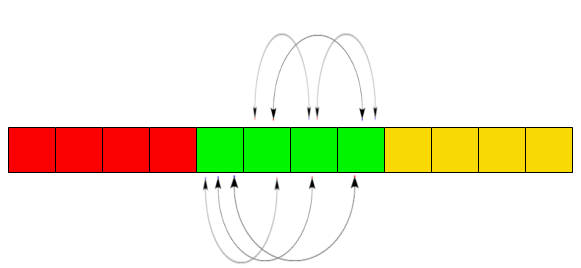
\includegraphics[width=1\linewidth]{array_proc_1_b_1}
\end{subfigure}\\ %
\begin{subfigure}{.3\textwidth}
  \centering
  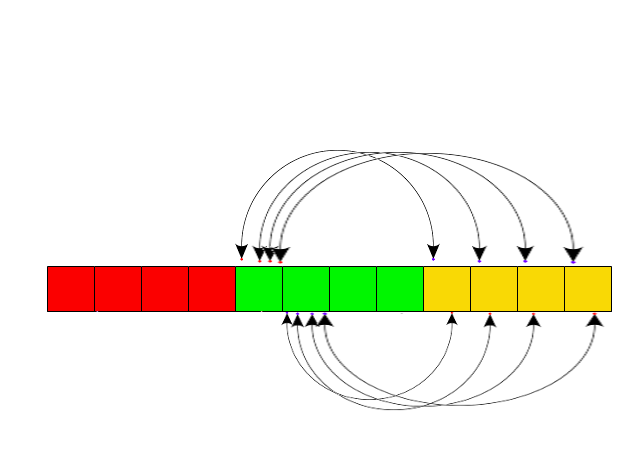
\includegraphics[width=1\linewidth]{array_proc_1_b_2}
\end{subfigure}
  \caption{Forces computed by Node 1 (8+6+8=22)}
  \label{fig:pr2}
\end{figure}
\FloatBarrier

\begin{figure}[!ht]
\centering
\begin{subfigure}{.3\textwidth}
  \centering
  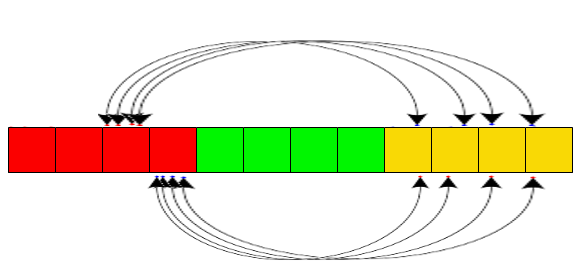
\includegraphics[width=1\linewidth]{array_proc_2_b_0}
\end{subfigure}%
\begin{subfigure}{.3\textwidth}
  \centering
  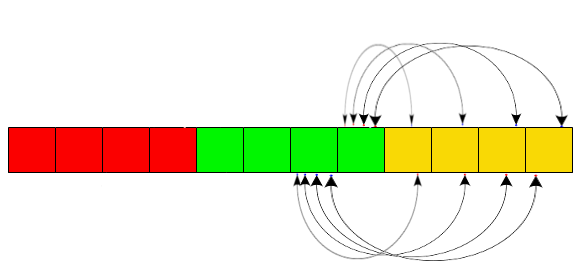
\includegraphics[width=1\linewidth]{array_proc_2_b_1}
\end{subfigure}\\ %
\begin{subfigure}{.3\textwidth}
  \centering
  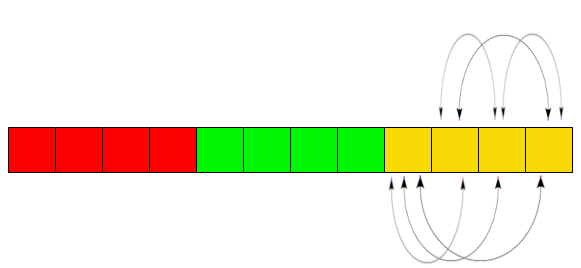
\includegraphics[width=1\linewidth]{array_proc_2_b_2}
\end{subfigure}
  \caption{Forces computed by Node 2 (8+8+6=22)}
  \label{fig:pr3}
\end{figure}
\FloatBarrier

Proceeding in this way, the forces between all pairs of bodies are calculated only one time per step. Each node computes the forces of 22 pairs. There are 3 nodes, so 3 times 22 is 66 that correspond to the number of possible pairs. No useful work is done. The approximated computational time is shown in the Equation \ref{eq:eq2}. The first O represents the computation of the forces between the assigned chunk's bodies and the bodies of other chunks, while the second O represents the computation of the forces among the assigned chunk's bodies.

\begin{equation} \label{eq:eq2}
\begin{split}
Complexity & = O(\lceil\frac{N}{P}\rceil * (\lceil\frac{N}{P}\rceil * \frac{1}{2}) * (P-1)) +  O(\sum_{i=1}^{\lceil\frac{N}{P}\rceil} {(\lceil\frac{N}{P}\rceil-i)})
\end{split}
\end{equation}

\subsubsection{Approach 2 - Forces repartition}
\label{sec:a2}
With this approach, the bodies are not taken into consideration, but only the forces to compute, resulting in a more simple and intuitive way to proceed. After calculating the total amount of forces to compute per step (Listing \ref{forces}), these can be simply distributed as shown in Listing \ref{fair}. The approximated computational time is shown in the Equation \ref{eq:eq3}.

\begin{lstlisting}[label=forces, caption=total amount of forces]
int forceCt = 0;
    for(i = 0; i < bodyCt; i++) {
        forceCt += i;
    }
\end{lstlisting}

\begin{equation} \label{eq:eq3}
\begin{split}
Complexity & = O(\lceil\frac{N^2}{P}\rceil)
\end{split}
\end{equation}

\subsubsection{Load imbalance}
\label{sec:b_rep}
As mentioned before, the load imbalance is a painful aspect of the parallel programming. If the total amount of work is perfectly divisible by the number of MPI processes, the two approaches are not so different, in fact, the number of forces calculated per machine is the same. The problems come out, when the work (bodies or forces) is not equally distributed. With the second approach, the inequity is simply reduced at the minimum. The maximum work difference between 2 nodes is of one force, that means less than 1\% of load imbalance if the assigned forces per machine are more than 100. To reach this bound with 16 MPI nodes, for example, 58 bodies (1653 forces) are sufficient. With the First approach is more difficult to balance the work, because the assigned number of bodies is different, and from one body the forces that exerts on all the others has to be calculated, that means a load imbalance of \textit{O(N)}. For this reason the second approach appeared more simple and efficient, so that it is adopted.


\subsection{The final solution}
\label{sec:final_sol}

\subsubsection{Communication VS Computation}
\label{sec:comm_comp}
The communication is a common bottleneck of lots of parallel implementations. The data exchange between nodes should be reduced at the minimum in order to obtain good performances. The problem with the N body algorithm is that at every step the updated information (positions, velocities) of all other bodies of the system is needed in order to correctly compute the forces of the assigned chunk.. To gain performances, a good compromise between the data exchange and the work to do on each node has to be found. In particular, the ratio \textit{computation/communication} should be maximized. 

\subsubsection{Approach one}
\label{sec:app_1}
Due to the fact that the force computation is the most expensive part of the algorithm and that as less data as possible should be exchanged, a good compromise is the following. The force (x, y) applied to a certain body is separated from the structure Body type, so at the beginning there are an array of N bodies and an array of N forces. As first thing, the bodies are broadcasted to all the nodes (\textit{MPI\_Bcast} Figure \ref{fig:A2}). After that, at each step, each node calculates the assigned forces, then with an \textit{MPI\_Allreduce} operation, all calculated arrays of N forces are summed (Figure \ref{fig:C2}) and as the last thing the velocities and positions for all the bodies are computed. Proceeding in this way, only an array of N elements containing the calculated forces is exchanged with the other nodes. The major problem with this approach, is that the positions and velocities of all the bodies are calculated in every node, that represents a duplication of work. An approximation of the complexity of a loop iteration and of the total amount of data exchanged per step is presented in Equations \ref{eq:comp_app1} and \ref{eq:com_app1}. In the first equation, the first \textit{O} represents the force computation step, the second the velocities computation and the third the positions computation. In the second equation, the \textit{2} represents the (x, y) values of the force.

\begin{figure}[ht]
\centering
\begin{minipage}{.5\textwidth}
  \centering
  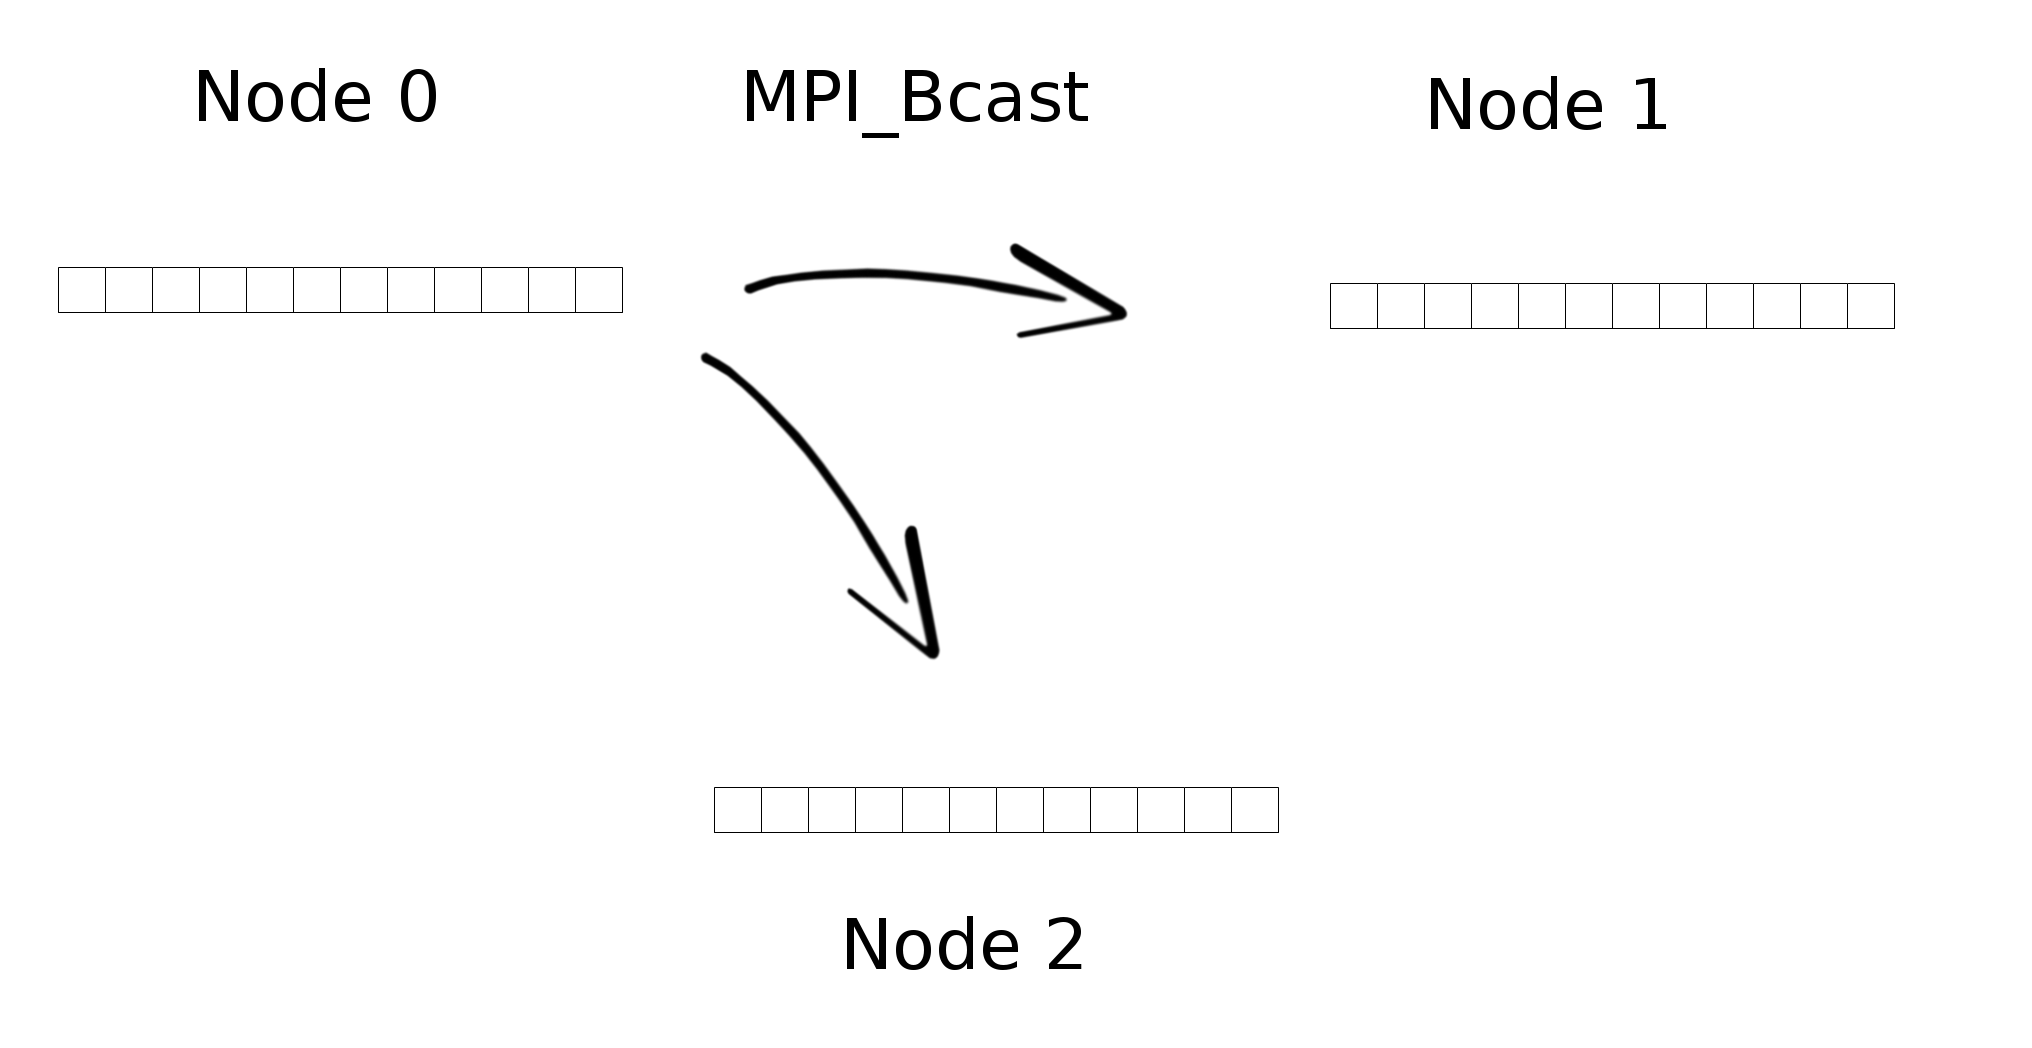
\includegraphics[width=\linewidth]{broadcast2}
  \caption{Broadcast the N bodies to all the nodes}
  \label{fig:A2}
\end{minipage}%
\begin{minipage}{.5\textwidth}
  \centering
  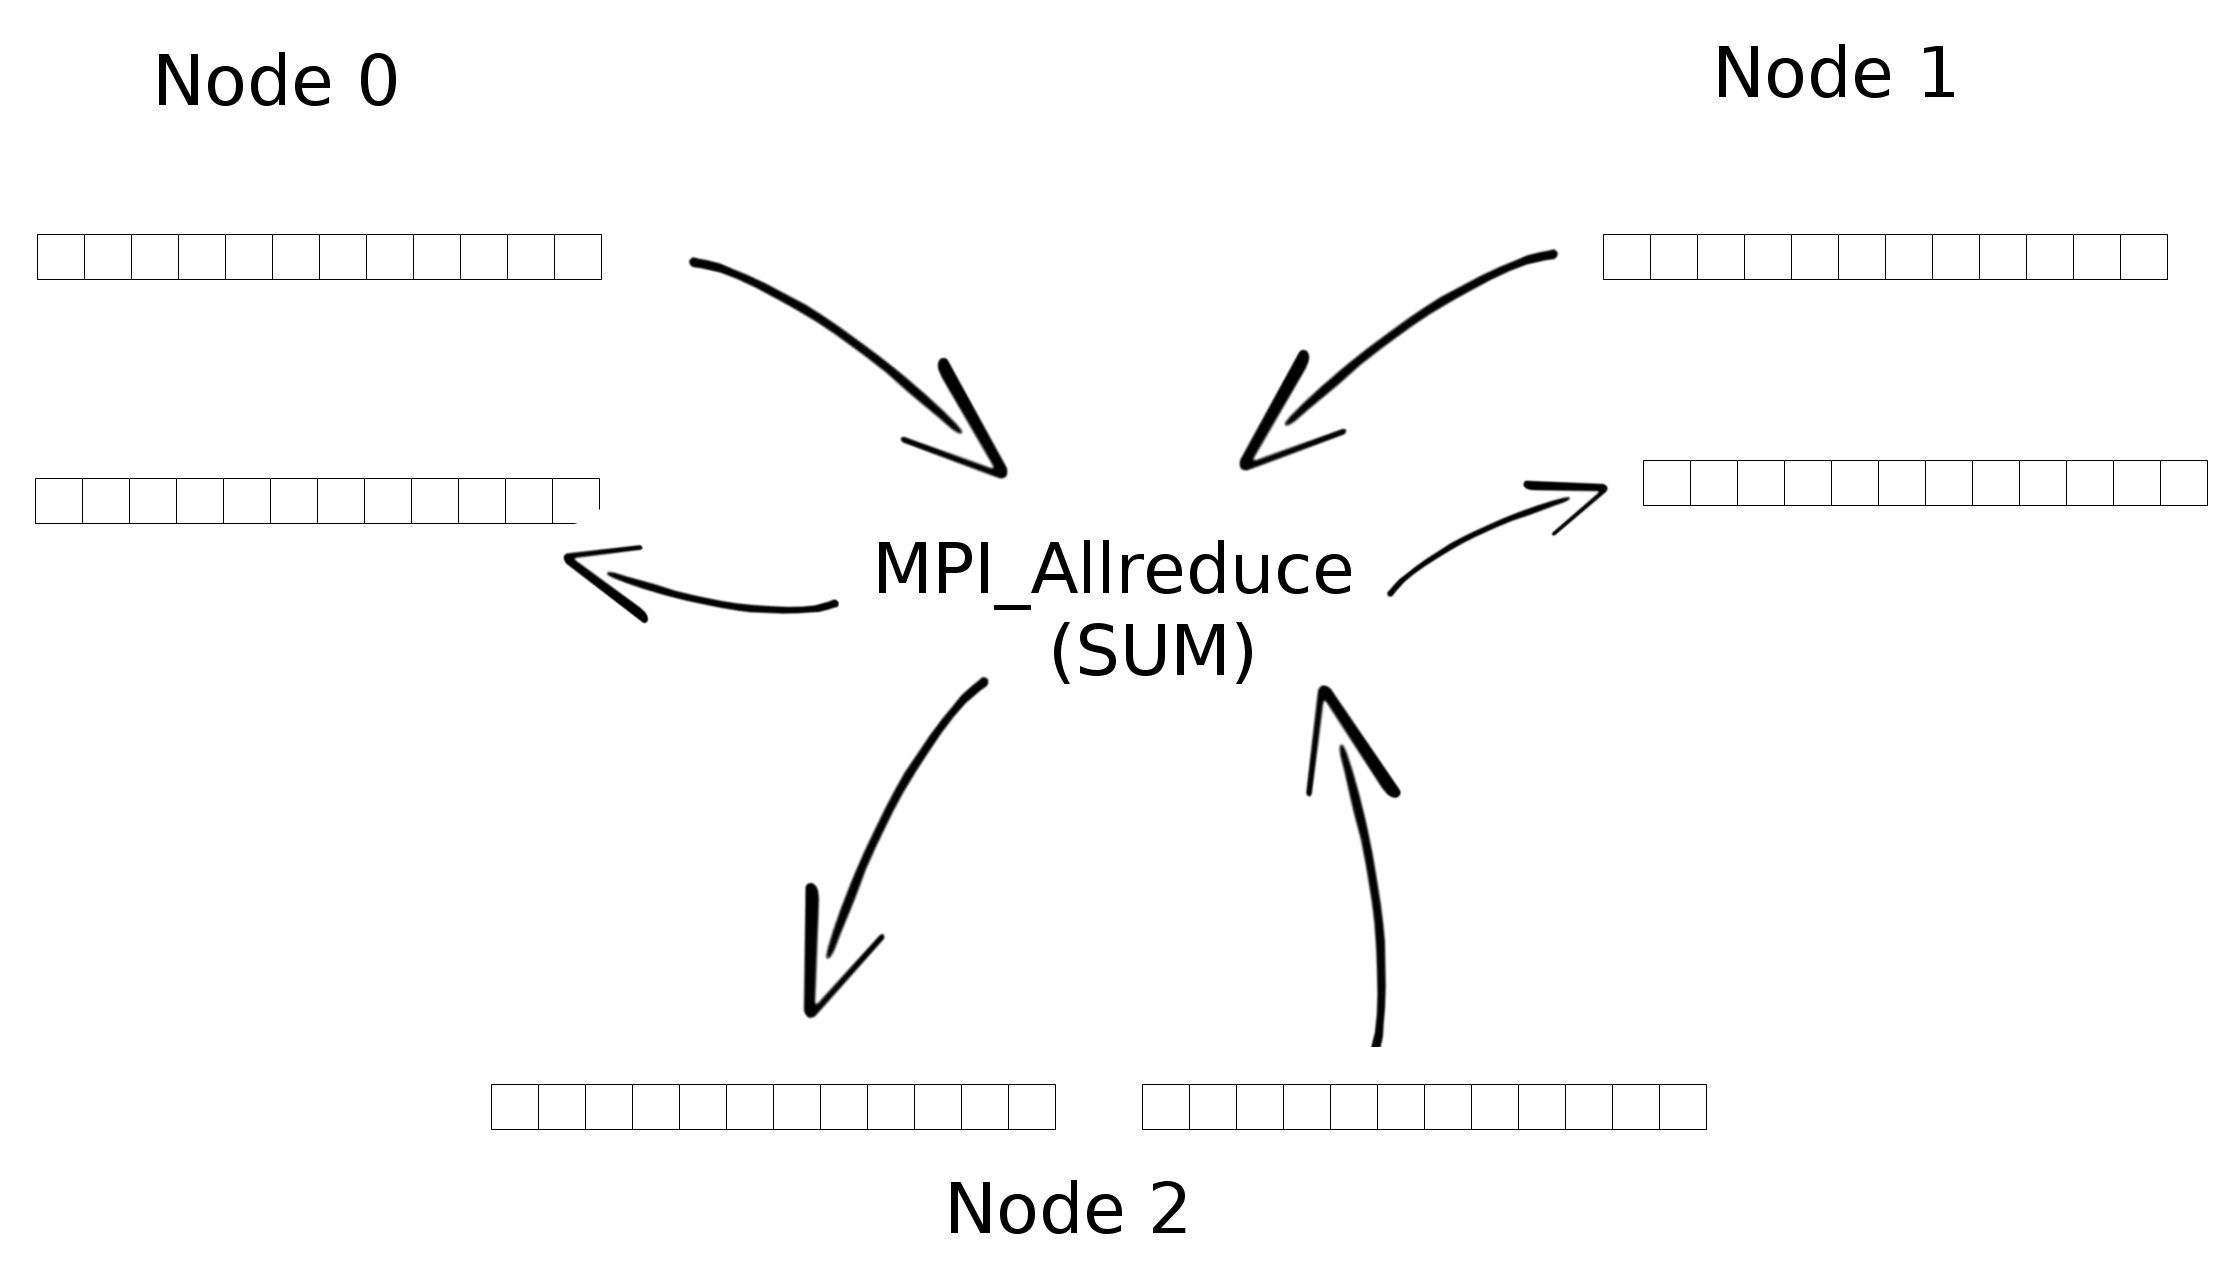
\includegraphics[width=\linewidth]{MPI_all_reduce}
  \captionof{figure}{The N forces reduction}
  \label{fig:C2}
\end{minipage}
\end{figure}
\FloatBarrier

\begin{equation} \label{eq:comp_app1}
\begin{split}
Complexity (per step) & = O(\lceil\frac{N^2}{P}\rceil)) + O(N) + O(N)
\end{split}
\end{equation}

\begin{equation} \label{eq:com_app1}
\begin{split}
Communication (per step) & = O(2*N)*sizeof(double)
\end{split}
\end{equation}

\subsubsection{Approach two}
\label{sec:app_2}
The aim of this approach, is to avoid the work duplication during the positions and velocities computation step. To calculate the force that two bodies exert on each other, at each step their mass, radius and position are needed. As first thing, the position (x, y) and the force of each body are separated from the structure Body type, so at the beginning there are an array of N bodies, an array of N positions and an array of N forces. 
The bodies and the positions are broadcasted to all the nodes and, after the calculation of the range of bodies and positions to assign to each node (with the method of Listing \ref{fair}), they are Scattered (Figure \ref{fig:sca}).
The force calculation step is the same as the one of the previous approach (calculation and \textit{MPI\_Allreduce}), afterwards the assigned positions and bodies are updated. Before starting another iteration, with an \textit{MPI\_Allgatherv} operation (Figure \ref{fig:posi}) the positions are gathered from all the nodes to all the nodes in order to have all the needed updated information for the next step. At the end, with an \textit{MPI\_Allgatherv} operation the final bodies are gathered from all the nodes to the "master" node that prints the results.
An approximation of the complexity of a loop iteration and of the total amount of data exchanged per step is presented in Equations \ref{eq:comp_app2} and \ref{eq:com_app2}. In the first equation, the first \textit{O} represents the force computation step, the second the velocity computation and the third the position computation. In the second equation, the \textit{4} represents the (x, y) values of the force and the (x, y) values of the position.

\begin{figure}[ht]
\centering
\begin{minipage}{.5\textwidth}
  \centering
  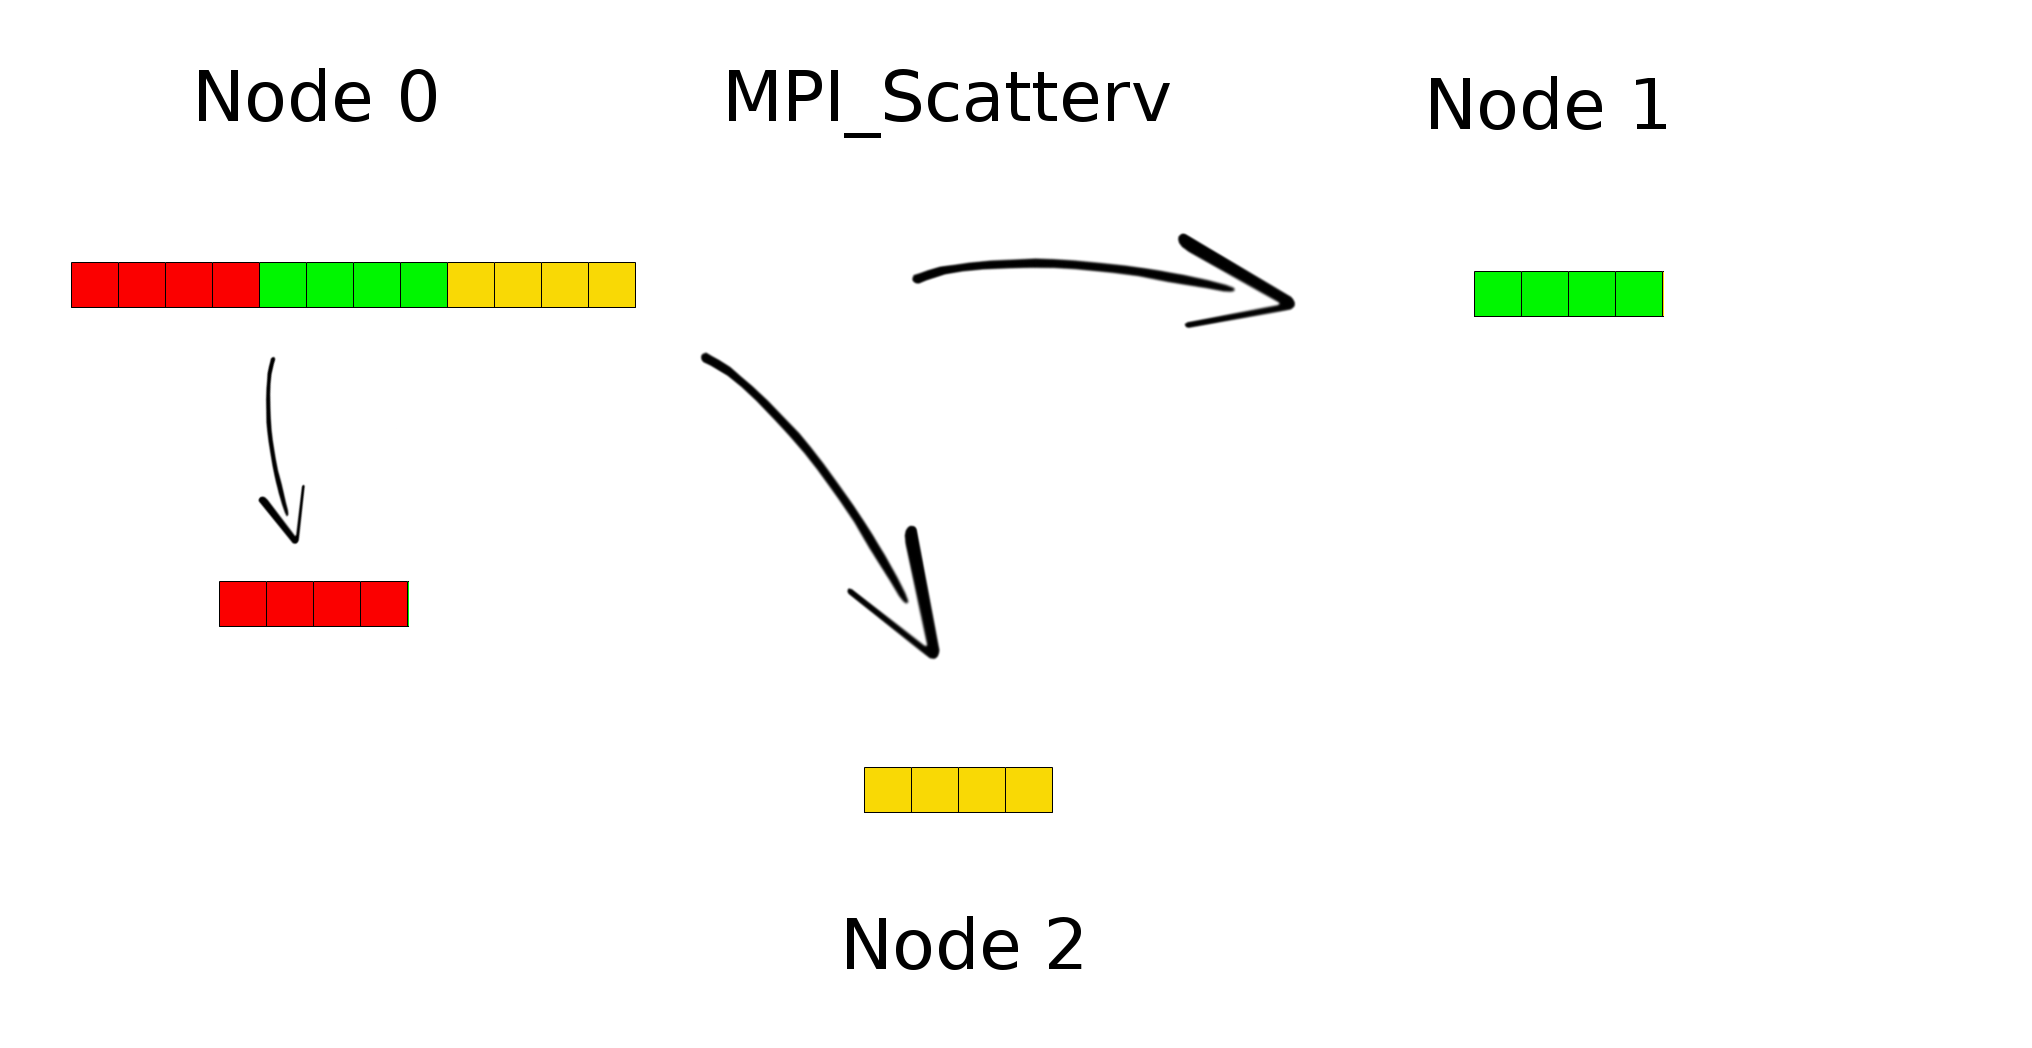
\includegraphics[width=\linewidth]{scatter}
  \caption{Distribute the N bodies to the nodes}
  \label{fig:sca}
\end{minipage}%
\begin{minipage}{.5\textwidth}
  \centering
  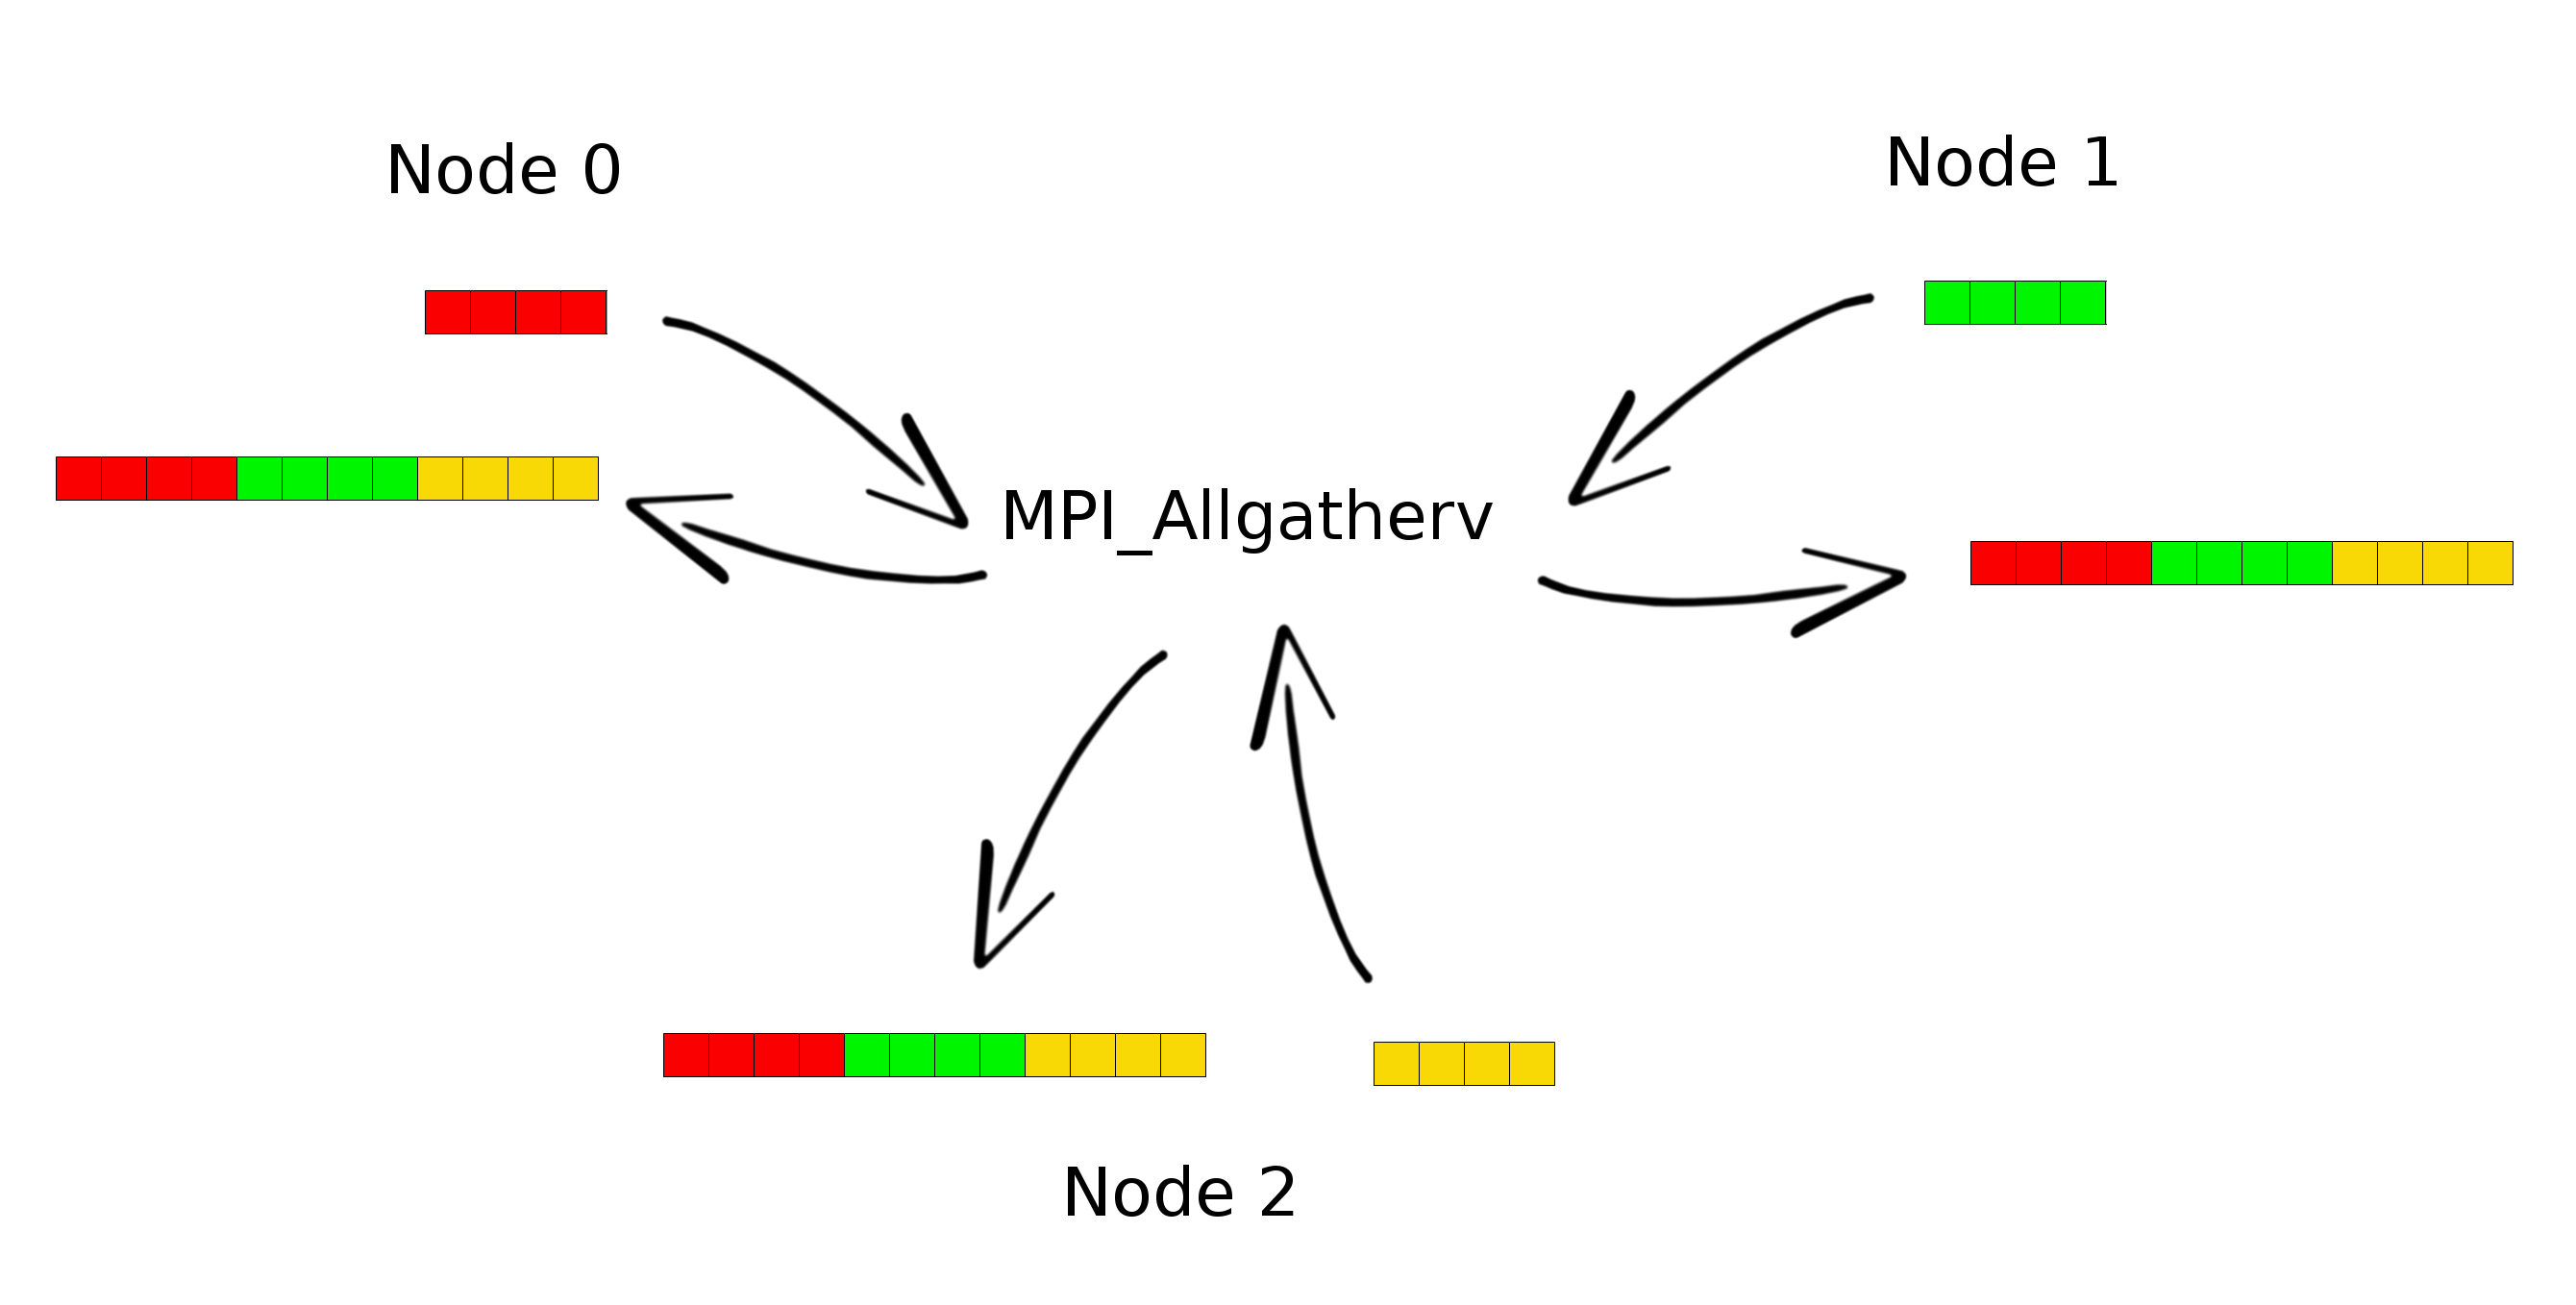
\includegraphics[width=\linewidth]{MPI_all_gather}
  \captionof{figure}{Collect updated positions from all the nodes}
  \label{fig:posi}
\end{minipage}
\end{figure}
\FloatBarrier



\begin{equation} \label{eq:comp_app2}
\begin{split}
Complexity (per step) & = O(\lceil\frac{N^2}{P}\rceil)) + O(\lceil\frac{N}{P}\rceil) + O(\lceil\frac{N}{P}\rceil)
\end{split}
\end{equation}

\begin{equation} \label{eq:com_app2}
\begin{split}
Communication (per step) & = O(4*N)*sizeof(double)
\end{split}
\end{equation}


\subsubsection{Solutions comparison}
\label{sec:sol_comp}
 
After a comparison of the two solutions for different size of inputs (steps and number of bodies), the second approach appears quite better, especially when the number of bodies is big, so that the cost of exchange more data is well covered. In Tables \ref{tab:t_app1} and \ref{tab:t_app2} (corresponding graphs in Figure \ref{fig:G1}) and in Tables \ref{tab:t_app3} and \ref{tab:t_app4} (corresponding graphs in Figure \ref{fig:G2}) are shown the execution times and speedups of the 2 approaches for different problem sizes. The lines in the graphs are almost overlapping, so that are not really clear the differences between the two approaches. Looking at the data in the tables, it is easy to understand that the second solution is better, especially when the size of the problem is big (10000 bodies) and for this reason it is the one adopted.
\\


\begin{minipage}[b]{.40\textwidth}
  \centering
\begin{tabular}{c|c|c}
\centering
\textbf{nodes/approaches} & \textbf{1} & \textbf{2} \\ \hline
\textbf{1}                & 474.974    & 474.974    \\ \hline
\textbf{2}                & 241.078    & 240.339    \\ \hline
\textbf{4}                & 123.869    & 123.335    \\ \hline
\textbf{8}                & 65.733     & 65.470     \\ \hline
\textbf{16}               & 37.264     & 37.427    
\end{tabular}
  \captionof{table}{256 bodies and 100000 iterations - Execution times}
  \label{tab:t_app1}
\end{minipage} \qquad
\begin{minipage}[b]{.40\textwidth}
  \centering
\begin{tabular}{c|c|c}
\textbf{nodes/approaches} & \textbf{1} & \textbf{2} \\ \hline
\textbf{2}                & 1.97       & 1.97       \\ \hline
\textbf{4}                & 3.83       & 3.85       \\ \hline
\textbf{8}                & 7.22       & 7.25       \\ \hline
\textbf{16}               & 12.74      & 12.69     
\end{tabular}
  \captionof{table}{256 bodies and 100000 iterations - Speedups}
  \label{tab:t_app2}
\end{minipage}

\begin{figure}[ht]
\begin{subfigure}{.55\textwidth}
  \centering
  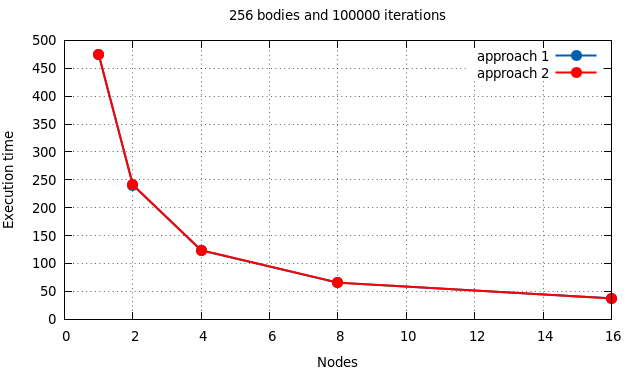
\includegraphics[width=1\linewidth]{results/256_100000_app}
\end{subfigure} %
\begin{subfigure}{.35\textwidth}
  \centering
  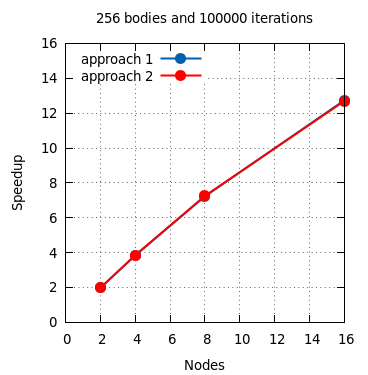
\includegraphics[width=1\linewidth]{results/256_100000_app_sp}
\end{subfigure} 
  \caption{Execution Time and Speedups of the two approaches with 256 bodies and 100000 iterations}
  \label{fig:G1}
\end{figure}
\FloatBarrier


\enspace

\begin{minipage}[b]{.40\textwidth}
  \centering
\begin{tabular}{c|c|c}
\textbf{nodes/approaches} & \textbf{1} & \textbf{2} \\ \hline
\textbf{1}                & 725.597    & 725.597    \\ \hline
\textbf{2}                & 362.751    & 361,145    \\ \hline
\textbf{4}                & 181.514    & 180.754    \\ \hline
\textbf{8}                & 90.954     & 90.637     \\ \hline
\textbf{16}               & 45.921     & 45.520    
\end{tabular}
  \captionof{table}{10000 bodies and 100 iterations - Execution times}
  \label{tab:t_app3}
\end{minipage} \qquad
\begin{minipage}[b]{.40\textwidth}
  \centering
\begin{tabular}{c|c|c}
\textbf{nodes/approaches} & \textbf{1} & \textbf{2} \\ \hline
\textbf{2}                & 2.0002     & 2.009      \\ \hline
\textbf{4}                & 3.997      & 4.014      \\ \hline
\textbf{8}                & 7.977      & 8.005      \\ \hline
\textbf{16}               & 15.80      & 15.94     
\end{tabular}
  \captionof{table}{10000 bodies and 100 iterations - Speedups}
  \label{tab:t_app4}
\end{minipage}


\begin{figure}[ht]
\begin{subfigure}{.55\textwidth}
  \centering
  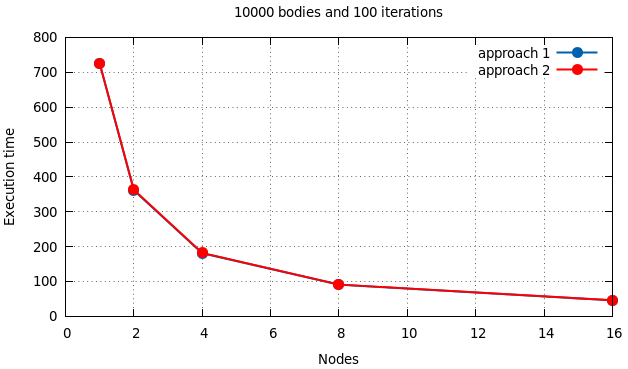
\includegraphics[width=1\linewidth]{results/10000_100_app}
\end{subfigure} %
\begin{subfigure}{.35\textwidth}
  \centering
  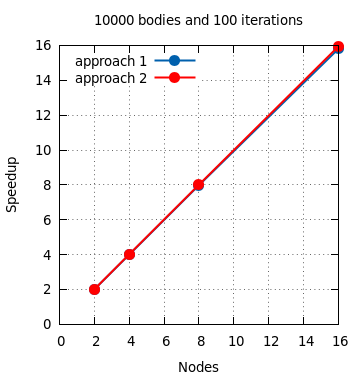
\includegraphics[width=1\linewidth]{results/10000_100_app_sp}
\end{subfigure}
  \caption{Execution Time and Speedups of the two approaches with 10000 bodies and 100 iterations}
  \label{fig:G2}
\end{figure}
\FloatBarrier


\subsubsection{Results}
\label{sec:res}
In this section the most interesting obtained results are reported. In Figure \ref{fig:R1} and Tables \ref{tab:R1_t1}, \ref{tab:R1_t2} we have an example with a big number of iterations (fixed) and different numbers of bodies (small). In Figure \ref{fig:R2} and Tables \ref{tab:R2_t1}, \ref{tab:R2_t2} we have an example with a small number of iterations (fixed) and different numbers of bodies (big). As we can see, the more we increase the size of the problem (number of bodies) and the more the implementation obtains good speedups. An interesting aspect is that in some cases, the speedup is superlinear (Figure \ref{fig:R2}, Table \ref{tab:R2_t2}, 1000 and 10000 bodies), due to the more cache and memory resources available on parallel systems. On a single machine, in fact, if the memory is not enough, there will be a lot of swapping and trashing, actions that are reduced having bigger available resources.
The aim of parallel programming is to deal with big size problems, so this implementation is good because the more we increase the number of bodies, the more the speedup is close to be linear. \\

\begin{figure}[ht]
\begin{subfigure}{.5\textwidth}
  \centering
  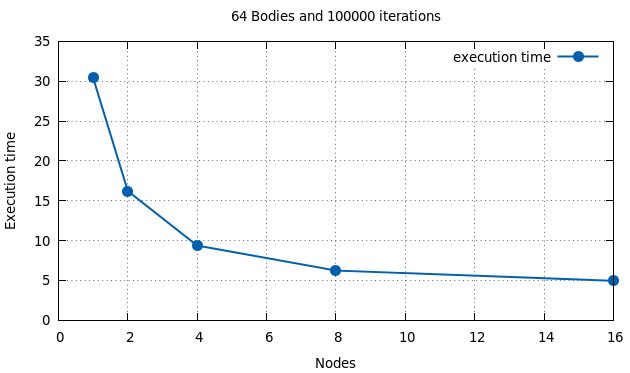
\includegraphics[width=1\linewidth]{results/64_100000}
\end{subfigure} %
\begin{subfigure}{.5\textwidth}
  \centering
  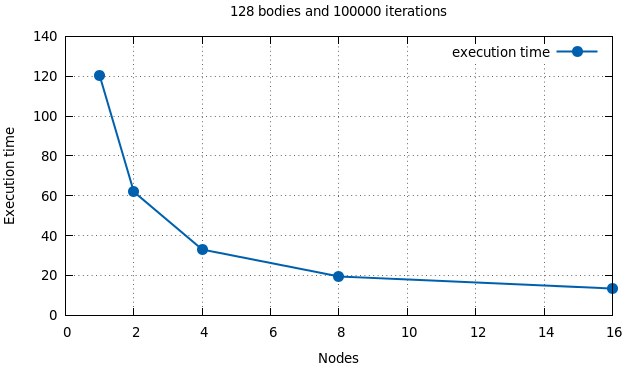
\includegraphics[width=1\linewidth]{results/128_100000}
\end{subfigure} \\ %
\begin{subfigure}{.5\textwidth}
  \centering
  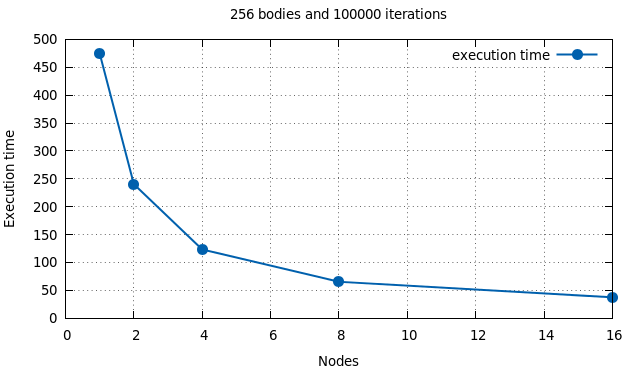
\includegraphics[width=1\linewidth]{results/256_100000}
\end{subfigure} %
\begin{subfigure}{.4\textwidth}
  \centering
  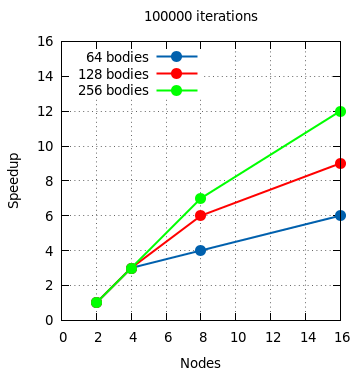
\includegraphics[width=1\linewidth]{results/100000_sp}
\end{subfigure}
  \caption{Execution Time and Speedups, 100000 iterations}
  \label{fig:R1}
\end{figure}
\FloatBarrier

\enspace


\begin{minipage}[b]{.40\textwidth}
  \centering
\begin{tabular}{c|c|c|c}
\textbf{nodes/bodies} & \textbf{64} & \textbf{128} & \textbf{256} \\ \hline
\textbf{1}            & 30.414      & 120.347      & 474.974      \\ \hline
\textbf{2}            & 16.463      & 61.939       & 240.339      \\ \hline
\textbf{4}            & 10.095      & 33,231       & 123.335      \\ \hline
\textbf{8}            & 7.336       & 19.477       & 65.470       \\ \hline
\textbf{16}           & 6.708       & 13.44        & 37.427      
\end{tabular}
  \captionof{table}{100000 iterations - Exec. times}
  \label{tab:R1_t1}
\end{minipage} \qquad
\begin{minipage}[b]{.40\textwidth}
  \centering
\begin{tabular}{c|c|c|c}
\textbf{nodes/bodies} & \textbf{64} & \textbf{128} & \textbf{256} \\ \hline
\textbf{2}            & 1.84        & 1.94         & 1.97         \\ \hline
\textbf{4}            & 3.012       & 3.62         & 3.85         \\ \hline
\textbf{8}            & 4.14        & 6.17         & 7.25         \\ \hline
\textbf{16}           & 4.53        & 8.95         & 12.69       
\end{tabular}
  \captionof{table}{100000 iterations - Speedups}
  \label{tab:R1_t2}
\end{minipage}

\begin{figure}[ht]
\begin{subfigure}{.5\textwidth}
  \centering
  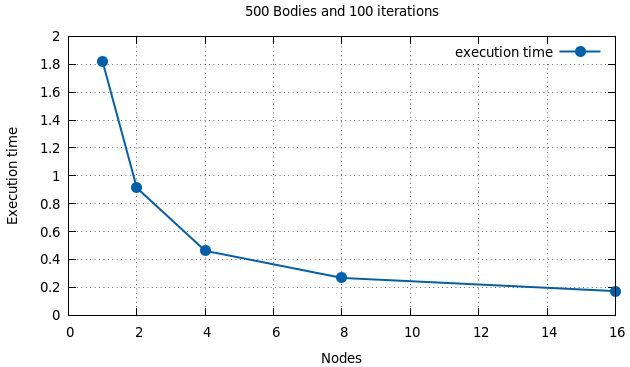
\includegraphics[width=1\linewidth]{results/500_100}
\end{subfigure} %
\begin{subfigure}{.5\textwidth}
  \centering
  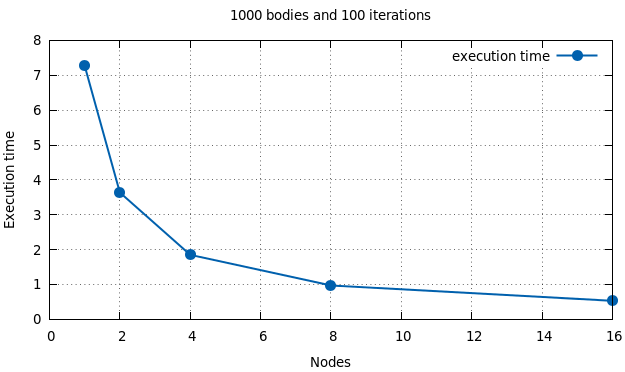
\includegraphics[width=1\linewidth]{results/1000_100}
\end{subfigure} \\ %
\begin{subfigure}{.5\textwidth}
  \centering
  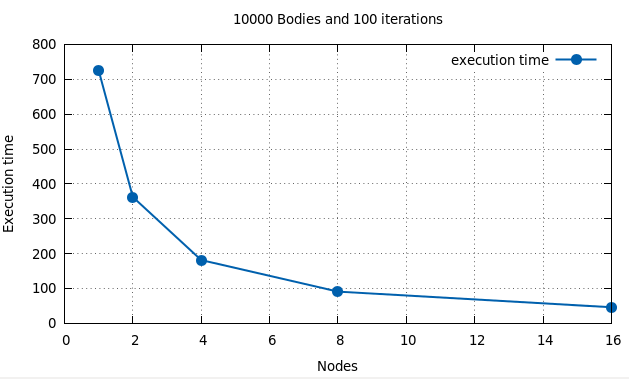
\includegraphics[width=1\linewidth]{results/10000_100}
\end{subfigure} %
\begin{subfigure}{.5\textwidth}
  \centering
  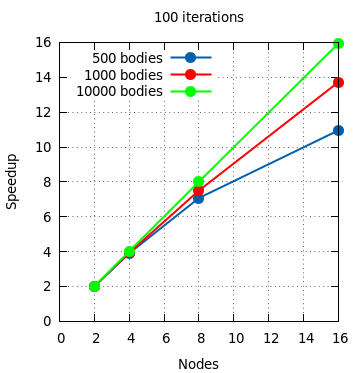
\includegraphics[width=1\linewidth]{results/100_sp}
\end{subfigure} 
  \caption{Execution Time and Speedups, 100 iterations}
  \label{fig:R2}
\end{figure}
\FloatBarrier

\begin{minipage}[b]{.40\textwidth}
  \centering
\begin{tabular}{c|c|c|c}
\textbf{nodes/bodies} & \textbf{500} & \textbf{1000} & \textbf{10000} \\ \hline
\textbf{1}            & 1.818        & 7.275         & 725.597        \\ \hline
\textbf{2}            & 0.911        & 3.636         & 361,145        \\ \hline
\textbf{4}            & 0.466        & 1.849         & 180.754        \\ \hline
\textbf{8}            & 0.257        & 0.969         & 90.637         \\ \hline
\textbf{16}           & 0.166        & 0.530         & 45.520        
\end{tabular}
  \captionof{table}{100 iterations - Exec. times}
  \label{tab:R2_t1}
\end{minipage} \qquad
\begin{minipage}[b]{.40\textwidth}
  \centering
\begin{tabular}{c|c|c|c}
\textbf{nodes/bodies} & \textbf{500} & \textbf{1000} & \textbf{10000} \\ \hline
\textbf{2}            & 1.99         & 2.0008        & 2.009          \\ \hline
\textbf{4}            & 3.90         & 3.93          & 4.014          \\ \hline
\textbf{8}            & 7.07         & 7.50          & 8.005          \\ \hline
\textbf{16}           & 10.95        & 13.72         & 15.94         
\end{tabular}
  \captionof{table}{100 iterations - Speedups}
  \label{tab:R2_t2}
\end{minipage}	

\vspace{8mm}

With the same number of bodies, but different number of iterations, the obtained speedup was more or less the same (Figure \ref{fig:R3} and Tables \ref{tab:R3_t1}, \ref{tab:R3_t2}). However, this is not surprising, because, for the same amount of bodies, there is the same work to do, but this is repeated for a different number of times.

\begin{figure}[ht]
\begin{subfigure}{.5\textwidth}
  \centering
  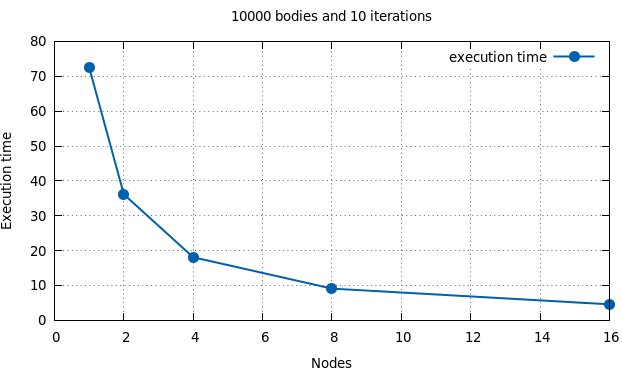
\includegraphics[width=1\linewidth]{results/10000_10}
\end{subfigure} %
\begin{subfigure}{.5\textwidth}
  \centering
  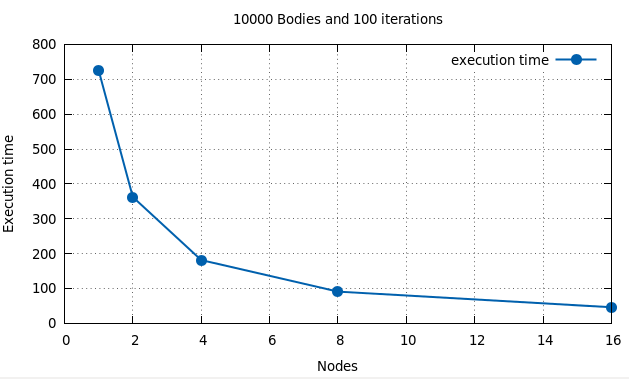
\includegraphics[width=1\linewidth]{results/10000_100}
\end{subfigure} \\ %
\begin{subfigure}{\textwidth}
  \centering
  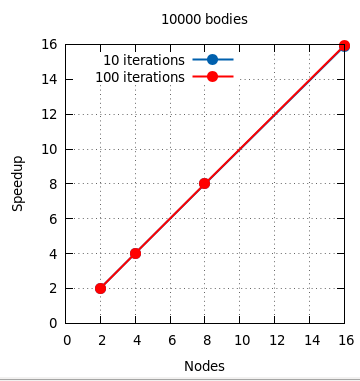
\includegraphics[width=.4\linewidth]{results/10000}
\end{subfigure} 
  \caption{Execution Time and Speedups, 1000 bodies}
  \label{fig:R3}
\end{figure}
\FloatBarrier


\begin{minipage}[b]{.40\textwidth}
  \centering
\begin{tabular}{|c|c|c|}
\hline
\textbf{nodes/iterations} & \textbf{10} & \textbf{100} \\ \hline
\textbf{1}                & 72.539      & 725.597      \\ \hline
\textbf{2}                & 36.111      & 361,145      \\ \hline
\textbf{4}                & 18.076      & 180.754      \\ \hline
\textbf{8}                & 9.076       & 90.637       \\ \hline
\textbf{16}               & 4.562       & 45.520       \\ \hline
\end{tabular}
  \captionof{table}{10000 bodies - Execution times}
  \label{tab:R3_t1}
\end{minipage} \qquad
\begin{minipage}[b]{.40\textwidth}
  \centering
\begin{tabular}{|c|c|c|}
\hline
\textbf{nodes/iterations} & \textbf{10} & \textbf{100} \\ \hline
\textbf{2}                & 2.008       & 2.009        \\ \hline
\textbf{4}                & 4.013       & 4.014        \\ \hline
\textbf{8}                & 7.99        & 8.005        \\ \hline
\textbf{16}               & 15.90       & 15.94        \\ \hline
\end{tabular}
  \captionof{table}{10000 bodies - Speedups}
  \label{tab:R3_t2}
\end{minipage}

\vspace{8mm}	

All the tests were performed on the Delft University of Technology (TUD) cluster (fs3.das4.tudelft.nl) and the execution times were measured using the "wall clock time". The data distribution and the data gathering, as being part of the application initialisation and de-initialisation, were not considered measuring the performance.

\section{Conclusions and Personal considerations}
\label{sec:con}
With the realized implementation, the speedups are close to be linear for big size problems and that means that is a good implementation. The MPI programming model dimonstrated to be optimal for this kind of works. At the beginning this model could appear hard to understand, especially for the MPI operations (e.g. MPI\_Allgatherv, MPI\_Scatterv), but after a short period of training it reveals all its power. Another interesting fact, is that programming using this library it could be useful, like in this particular project case, to have more than one implementation in order to compare the results and outline any weaknesses.  

		
\printbibliography 

\end{document}